Figure~\ref{fig:deconv} shows the
serial interval and incubation period distributions
from \cite{Du2020} and \cite{Lauer2020} respectively,
and the generation time distribution estimated via the proposed method.
The \mle parameters of $\hat{G}(\tau\mid\theta)$ were:
shape ${\alpha = 1.813}$ and scale ${\beta = 2.199}$,
yielding $\hat{S}(\tau\mid\theta^*)$
that reasonably approximated the target $S(\tau)$.
\par
Comparing the estimated generation time to published serial interval distributions
(Figure~\ref{fig:distr-refs}) showed the following.
The mean generation time of $3.99$ was similar to
the mean serial interval of $3.96$
based on the negative-permitting distribution \cite{Du2020},
but shorter than mean serial interval based on non-negative distributions,
such as $5.12$ in \cite{Zhang2020} and $4.7$ in \cite{Nishiura2020}.
The \sd of the generation time distribution was smaller at $2.96$
than the \sd of the negative permitting serial interval at $4.75$ \cite{Du2020},
but similar to the \sd of the non-negative serial interval distributions,
including $2.69$ in \cite{Zhang2020} and $2.9$ in \cite{Nishiura2020}.
\par
\begin{figure}
  \centering
  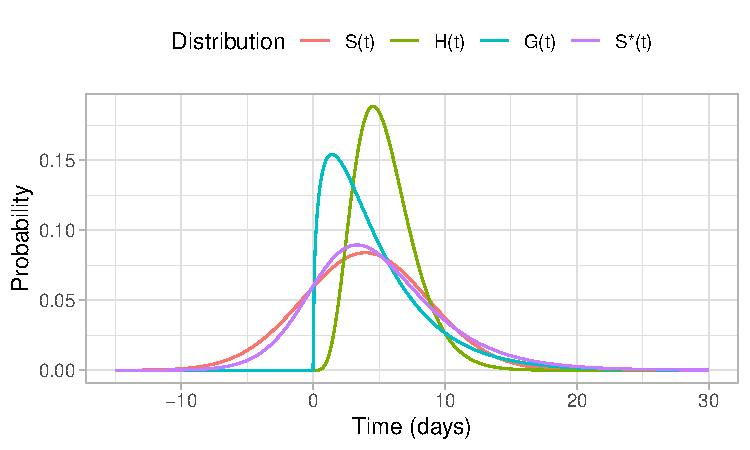
\includegraphics[width=\linewidth]{deconv}
  \caption{Recovered generation time distribution
    $\hat{G}(\tau\mid\theta^*)$
    based on \mle approximation of the serial interval distribution
    $S(\tau)$ by $\hat{S}(\tau\mid\theta^*)$
    and the incubation period distribution $H(\tau)$.}
  \label{fig:deconv}
\end{figure}
\par
Figure~\ref{fig:Re} shows
$\Re(t)$ for \covid in \gta, Canada
based on reported cases and estimated using
the generation time distribution versus
selected serial interval distributions reported in the literature.%
\footnote{Generation time and serial interval distributions
  are also illustrated in Figure~\ref{fig:distr-refs}.}
The $\Re(t)$ based on non-negative serial interval distribution was higher
versus $\Re(t)$ using the estimated generation time distribution
(e.g.\ using \cite{Zhang2020}:\
\rvalue{R-2020-03-16-S(t)-[NN]-Zhang-2020} vs
\rvalue{R-2020-03-16-G(t)-[this]} on March~16; and
\rvalue{R-2020-04-13-S(t)-[NN]-Zhang-2020} vs
\rvalue{R-2020-04-13-G(t)-[this]} on April~13).
Higher $\Re(t)$ can be attributed to
longer mean serial interval under non-negative distributions
versus the estimated mean generation time,
since inferred $\Re(t)$ must be higher
to compensate for longer delay between infections.%
\footnote{Relative differences in $\Re(t)$ between input distributions  %SM: good!
  are ``flipped'' after $\Re < 1$,
  since a longer delay between infections has opposite implications for $\Re(t)$
  in the context of a shrinking versus growing epidemic.}
By contrast, the $\Re(t)$ estimated using
a negative-permitting serial interval distribution
was the smallest of all three approaches
(e.g.\ using \cite{Du2020}:\
\rvalue{R-2020-03-16-S(t)-[NP]-Du-2020} on March~16; and
\rvalue{R-2020-04-13-S(t)-[NP]-Du-2020} on April~13).
In this case, lower $\Re(t)$ can be attributed to
increased variance in the negative-permitting serial interval distribution
versus in the generation time distribution,
as shown in \cite{Britton2019}.
\par
\begin{figure}[h]
  \centering
  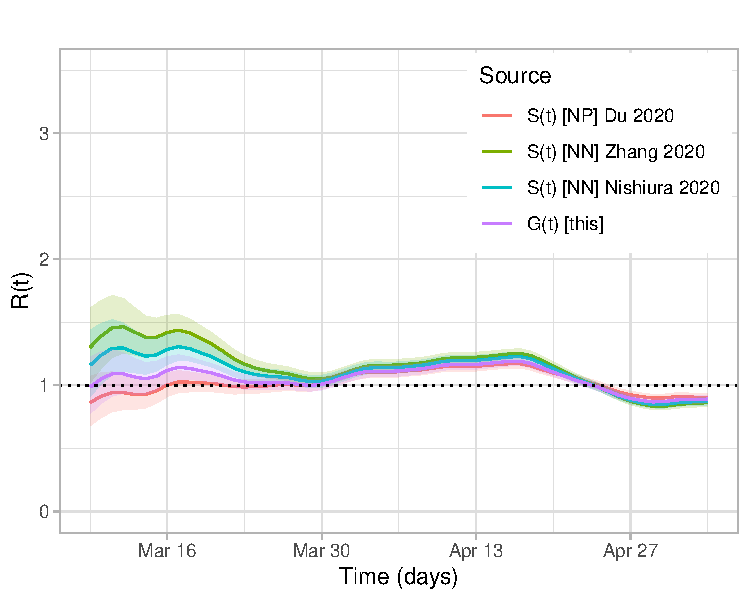
\includegraphics[width=\linewidth]{Re}
  \caption{$\Re(t)$ of \covid in \gta using
    serial interval versus generation time}
  \label{fig:Re}
  \floatfoot{Notation ---
    $S(\tau)$:~serial interval;
    $G(\tau)$:~generation time;
    [NP]:~negative-permitting;
    [NN]:~non-negative.
    See Figure~\ref{fig:Re-zoom}
    for zoom-in of later dates.
  }
\end{figure}